\section{块邻近梯度（BPG）}
\label{sec:block-bpg}

许多目标是光滑项加上按块可分的非光滑项，例如最小二乘加$\ell_1$正则。接下来要弄清：怎样在一块上同时利用光滑项的梯度和非光滑项的结构，并判断算法何时可以停下来？

设目标是式~\eqref{eq:block-composite}的形式，$g_J$是适当、下半连续的凸函数。第~\ref{chap:nonsmooth-composite-optimization}章已经对完整变量建立了邻近梯度法，这里集中说明分块之后什么地方变了：可分性让邻近映射能逐块计算，步长由块常数决定，残差的含义也不同。第~\ref{sec:block-apcg}小节的APCG是在同样的复合结构上另配了加速递推。

\subsection{块邻近更新}
\label{sec:block-prox-update}

\paragraph{主要思想}
在块$J$上，用二次上界代替光滑项，原样保留非光滑项，得到模型
\begin{equation}
 \begin{aligned}
 u_J(\bm{z};\bm{x})={}&f(\bm{x})+\langle\nabla_Jf(\bm{x}),\bm{z}-\bm{x}_J\rangle+\frac{L_J}{2}\lVert\bm{z}-\bm{x}_J\rVert_2^2\\
 &+g_J(\bm{z})+\sum_{i\neq J}g_i(\bm{x}_i).
 \end{aligned}
 \label{eq:block-prox-model}
\end{equation}

其中只有$\bm{z}$是变量。对前三项配方，最小化$u_J$等价于
\[
 \min_{\bm{z}}\ g_J(\bm{z})+\frac{L_J}{2}\Bigl\lVert\bm{z}-\Bigl(\bm{x}_J-\frac{1}{L_J}\nabla_Jf(\bm{x})\Bigr)\Bigr\rVert_2^2 ,
\]

这正是邻近映射的定义。于是\term{块邻近梯度}（block proximal gradient，BPG）的更新是块梯度步接邻近映射：
\begin{equation}
 \bm{x}_J^{+}=\operatorname{prox}_{g_J/L_J}\Bigl(\bm{x}_J-\frac{1}{L_J}\nabla_Jf(\bm{x})\Bigr).
 \label{eq:block-prox}
\end{equation}
$g_J$是闭凸集$\bm{C}_J$的示性函数时，邻近映射就是到$\bm{C}_J$的投影，式~\eqref{eq:block-prox}成为块投影梯度步，第~\ref{sec:block-coupling}小节的乘积可行域由此纳入同一框架。

\paragraph{完整目标不增}
步长取块常数的倒数，邻近映射精确计算，就有下面的下降量。

\begin{lemma}[块邻近步的下降量]
\label{lem:block-prox-descent}
设$f$可微且满足定义~\ref{def:block-smooth}，$g_J$是适当、下半连续的凸函数，$F(\bm{x})<+\infty$。按式~\eqref{eq:block-prox}更新块$J$，其余块不变，得到$\bm{x}^{+}$。则
\begin{equation}
 F(\bm{x})-F(\bm{x}^{+})\geq\frac{L_J}{2}\lVert\bm{x}_J^{+}-\bm{x}_J\rVert_2^2 .
 \label{eq:block-prox-descent}
\end{equation}
\end{lemma}

\begin{proof}
由式~\eqref{eq:block-quadratic-upper}，$u_J$是块上界，所以$F(\bm{x}^{+})\leq u_J(\bm{x}_J^{+};\bm{x})$。模型的光滑部分带系数$L_J/2$，$g_J$凸，所以$u_J$关于$\bm{z}$是$L_J$强凸的。

$\bm{x}_J^{+}$是$u_J$的最小点，强凸性给出：对任意$\bm{z}$，
\[
 u_J(\bm{z};\bm{x})\geq u_J(\bm{x}_J^{+};\bm{x})+\frac{L_J}{2}\lVert\bm{z}-\bm{x}_J^{+}\rVert_2^2 .
\]

取$\bm{z}=\bm{x}_J$，并由$u_J(\bm{x}_J;\bm{x})=F(\bm{x})$，得到
\[
 F(\bm{x})\geq u_J(\bm{x}_J^{+};\bm{x})+\frac{L_J}{2}\lVert\bm{x}_J-\bm{x}_J^{+}\rVert_2^2\geq F(\bm{x}^{+})+\frac{L_J}{2}\lVert\bm{x}_J-\bm{x}_J^{+}\rVert_2^2 .
\]
\end{proof}

若步长取得比$1/L_J$大，$u_J$就可能不再是上界，下降量不再有保证。这里的“精确”也不是可有可无的条件：邻近子问题解得不准时，要按第~\ref{sec:block-inexact}小节计入误差。

\paragraph{计算过程：套索的单坐标更新}
考虑套索问题，$\gamma>0$，取最小二乘的光滑项和$\ell_1$正则：
\[
 F(\bm{x})=\frac12\lVert\bm{A}\bm{x}-\bm{b}\rVert_2^2+\gamma\lVert\bm{x}\rVert_1 .
\]
取坐标为块，$g_j=\gamma\lvert\cdot\rvert$可分，$\gamma\lvert\cdot\rvert/L_j$的邻近映射是软阈值
\begin{equation}
 S_{\tau}(v)=\operatorname{sign}(v)\max\{\lvert v\rvert-\tau,\,0\},\qquad \tau=\frac{\gamma}{L_j}.
 \label{eq:block-soft-threshold}
\end{equation}
于是式~\eqref{eq:block-prox}成为
\begin{equation}
 x_j^{+}=S_{\gamma/L_j}\Bigl(x_j-\frac{1}{L_j}\bm{a}_j^\top\bm{r}\Bigr),\qquad L_j=\lVert\bm{a}_j\rVert_2^2 .
 \label{eq:block-lasso-update}
\end{equation}
这时光滑项的条件函数是抛物线，上界等于它，式~\eqref{eq:block-lasso-update}也是精确块解。

\needspace{6\baselineskip}
\paragraph{变量}
\begin{itemize}
 \item $\bm{x}$：当前系数；$\bm{r}=\bm{A}\bm{x}-\bm{b}$：残差，每次更新后维护。
 \item $L_j$：各列的平方范数，事先算好；$\gamma$：正则系数。
\end{itemize}

\paragraph{初始化}
下面用与前面相同的$\bm{A}$，并取以下数据进行演示：
\[
 \bm{b}=(4,2,-1),\qquad \gamma=1,\qquad \bm{x}^{(0)}=(3,4).
\]
于是$L_1=L_2=2$，阈值$\tau=\tfrac12$，初始残差$\bm{r}=(3,1,5)$，目标值$F=24.5$。

\paragraph{每轮更新}
循环取坐标$j=1,2$，每次按式~\eqref{eq:block-lasso-update}更新$x_j$，再更新残差$\bm{r}\leftarrow\bm{r}+(x_j^{+}-x_j)\bm{a}_j$。

\begin{enumerate}
 \item 第一轮，$j=1$：$\bm{a}_1^\top\bm{r}=4$，软阈值的输入是$3-2=1$，于是
 \[
  x_1=0.5,\qquad \bm{r}=(0.5,-1.5,5),\qquad F=18.25 .
 \]
 \item 第一轮，$j=2$：$\bm{a}_2^\top\bm{r}=5.5$，输入是$4-2.75=1.25$，于是
 \[
  x_2=0.75,\qquad \bm{r}=(-2.75,-1.5,1.75),\qquad F=7.6875 .
 \]
 \item 第二轮，$j=1$：$\bm{a}_1^\top\bm{r}=-4.25$，输入是$0.5+2.125=2.625$，于是
 \[
  x_1=2.125,\qquad \bm{r}=(-1.125,0.125,1.75),\qquad F=5.046875 .
 \]
 \item 第二轮，$j=2$：$\bm{a}_2^\top\bm{r}=0.625$，输入是$0.75-0.3125=0.4375$，小于阈值，于是
 \[
  x_2=0,\qquad \bm{r}=(-1.875,0.125,1),\qquad F=4.390625 .
 \]
 \item 第三轮，$j=1$：$\bm{a}_1^\top\bm{r}=-1.75$，输入是$2.125+0.875=3$，于是
 \[
  x_1=2.5,\qquad \bm{r}=(-1.5,0.5,1),\qquad F=4.25 .
 \]
 \item 第三轮，$j=2$：$\bm{a}_2^\top\bm{r}=-0.5$，输入是$0+0.25=0.25$，仍小于阈值，$x_2$保持为$0$。
\end{enumerate}

此时两个坐标都不再变化，迭代结束，最终得到$\bm{x}=(2.5,0)$，$F=4.25$。图~\ref{fig:block-soft-threshold}(a)是软阈值函数，(b)是这条路径。第二轮之后$x_2$被压到$0$并留在那里，这就是$\ell_1$正则产生稀疏解的方式。

\begin{BookInlineFigure}
  \centering
  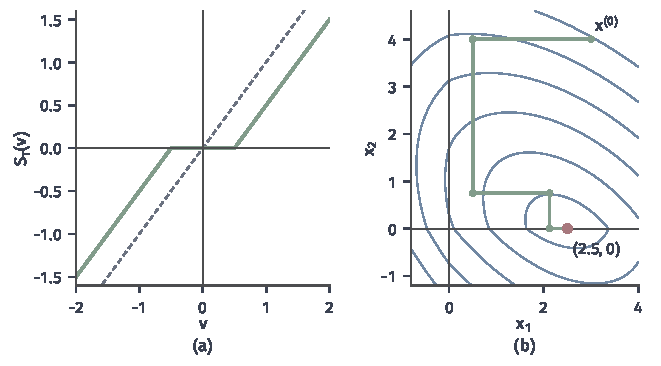
\includegraphics[width=112mm]{figures/05-optimization/04-block-optimization/matplotlib/block-soft-threshold/figure.pdf}
  \caption{套索的坐标更新。(a)软阈值函数$S_{1/2}(v)$（绿），灰色虚线是恒等映射，$\lvert v\rvert\leq\tfrac12$的输入被压成$0$。(b)文中的例子：蓝色是复合目标的等高线，绿色折线是循环更新的路径，第二轮把$x_2$压到坐标轴上，红点是解$(2.5,0)$。}
  \label{fig:block-soft-threshold}
\end{BookInlineFigure}

\paragraph{可分性的边界}
上面每一步能单独计算，靠的是非光滑项能拆成$\sum_jg_j(x_j)$。对式~\eqref{eq:block-nonsmooth-example}这样的不可分项，把一块的条件函数写出来仍是可以的，比如固定$v$后对$u$的邻近子问题，但它的结果依赖其他块，算法也就可能如第~\ref{sec:block-coupling}小节那样停滞。逐块计算的前提和逐块最优性能合成整体驻点的前提，是同一个可分性。

\subsection{块邻近残差}
\label{sec:block-prox-residual}

\paragraph{要回答的问题}
光滑时用偏梯度判断一块是否调好了。有非光滑项时偏梯度不再归零，比如解$(2.5,0)$处第二个坐标的偏导数是$-0.5$，不是$0$，该坐标却已经最优。需要一个既能处理非光滑项又能计算的量。

\begin{definition}[块梯度映射]
\label{def:block-gradient-mapping}
设$\alpha>0$，定义块$J$的\term{块梯度映射}（block gradient mapping）为
\begin{equation}
 \bm{G}_J(\bm{x})=\frac{1}{\alpha}\Bigl(\bm{x}_J-\operatorname{prox}_{\alpha g_J}\bigl(\bm{x}_J-\alpha\nabla_Jf(\bm{x})\bigr)\Bigr).
 \label{eq:block-gradient-mapping}
\end{equation}
\end{definition}

它是块邻近步的位移除以步长。$g_J\equiv0$时就是偏梯度$\nabla_Jf(\bm{x})$，所以它是偏梯度的自然推广。

\paragraph{全部为零即复合驻点}
由邻近映射的最优性条件可以读出这个量的含义。记$\bm{p}=\operatorname{prox}_{\alpha g_J}(\bm{v})$，则$\bm{p}$满足$(\bm{v}-\bm{p})/\alpha\in\partial g_J(\bm{p})$，其中$\partial g_J$是次微分。取$\bm{v}=\bm{x}_J-\alpha\nabla_Jf(\bm{x})$，$\bm{G}_J(\bm{x})=\bm{0}$就是$\bm{p}=\bm{x}_J$，代入得到
\[
 -\nabla_Jf(\bm{x})\in\partial g_J(\bm{x}_J).
\]

反过来，若上式成立，$\bm{x}_J$满足邻近子问题的最优性条件，邻近映射的解唯一，所以$\bm{p}=\bm{x}_J$。

因此全部块的映射同时为零，等价于每块都有$-\nabla_Jf(\bm{x})\in\partial g_J(\bm{x}_J)$。由$g$按块可分，次微分是各块次微分的乘积，上面$B$个包含关系合起来就是
\begin{equation}
 \bm{0}\in\nabla f(\bm{x})+\partial g(\bm{x}).
 \label{eq:block-composite-stationary}
\end{equation}
这是复合目标的驻点条件。$f$凸时，由引理~\ref{lem:block-joint-convex}的论证，它也是全局最优条件。

\paragraph{刚更新块的残差}
实际运行中还有一个容易出错的地方：不要拿刚更新块的残差代替完整残差。例中取$\alpha=\tfrac12$，看前两步的残差，其中$\bm{G}_J$的值都按更新后的点重新计算：
\[
 \begin{aligned}
 \bm{x}=(3,4):&\quad G_1=5,\quad G_2=8,\\
 \bm{x}=(0.5,4):&\quad G_1=0,\quad G_2=6.5,\\
 \bm{x}=(0.5,0.75):&\quad G_1=-3.25,\quad G_2=0.
 \end{aligned}
\]
第二行刚更新了$x_1$，$G_1$变成$0$。但第三行更新$x_2$之后，$G_1$又变成了$-3.25$：$x_1$在新的$x_2$下不再是最优的。

一块的残差只反映这一块在当时的状况，其他块一变，先前算出的残差就过期了。完整驻点残差要求所有块在同一点上重新计算，停止准则应当用它，或者至少在一轮结束后重算一次。

图~\ref{fig:block-residual-stale}对比了两个量。黄点是每次更新前对被更新块算出的残差，绿线是当时所有块的完整残差。黄点常常比绿线小一到两个数量级，个别的还接近零，这时只看单块残差就会过早停止。

\begin{BookInlineFigure}
  \centering
  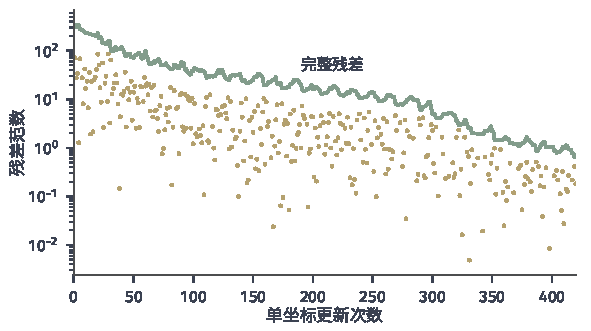
\includegraphics[width=100mm]{figures/05-optimization/04-block-optimization/matplotlib/block-residual-stale/figure.pdf}
  \caption{单块残差与完整残差。$N=60$、$n=30$的套索问题（列之间相关，$\gamma=2$），循环单坐标更新$14$轮。绿线是全部块的残差范数，黄点是每次被更新那一块在更新前的残差绝对值（$\alpha=1/L_j$）。残差为零的点因对数坐标未画出。}
  \label{fig:block-residual-stale}
\end{BookInlineFigure}
